\chapter{Elektromagnetisme} \label{chap:el}

\section{Introduktion}

I mekanik arbejdes der med spørgsmålet om, hvordan et legeme bevæger sig, når det bliver påvirket af en kraft. Generelt eksisterer der kun \emph{fire} forskellige kræfter i naturen, som vi kender til. Disse er tyngdekraften, den stærke kernekraft, den svage kernekraft og den elektromagnetiske kraft. Hvis du allerede har været igennem klassisk mekanik i fysik, kan du måske stille dig selv spørgsmålene: Hvor er normalkraften? Hvad med friktion? Hvad med kraften som stopper en bold fra at falde gennem jorden? Hvad med de kemiske kræfter som binder molekyler sammen? Det korte svar er, at disse allesammen er \emph{elektromagnetiske}. Det er altså ikke en stor overdrivelse, at vi kan se og føle på grund af elektromagnetismen. Lys er en elektromagnetisk bølge, og når vi kan mærke et objekt, er det fordi, vi føler den elektromagnetiske frastødning mellem os og det.

Fra afstandene mellem atomer og op til afstande ude i rummet er den elektromagnetiske kraft fuldstændig dominerende. De to kernekræfter har så kort rækkevidde, at vi ikke mærker dem i dagligdagen, og tyngdekraften har stort set ingen effekt i atomernes verden, da masserne er for små. Til gengæld, hvis vi dykker ind i selve atomet, er det den stærke kernekraft, som holder protoner og neutroner sammen, og mellem himmellegemer er det tyngdekraften, som er størst. Elektromagnetismen er derfor vigtig at forstå, når vi arbejder med alt mellem atomer og planeter.

\section{Elektrisk ladning} \label{sec:ladning}
\begin{enumerate}
    \item \textit{Ladning kommer i to varianter}, som vi definerer til at være ``plus'' og ``minus''. Vi kalder dem dette, fordi deres påvirkning empirisk set ``går ud med hinanden'' -- hvis to ladninger $+q$ og $-q$ placeres oven på hinanden, vil det elektrisk set være det samme, som hvis der ikke var nogle ladninger overhovedet. Disse fakta er måske en smule åbenlyse, men hvordan ville tingene måske opføre sig, hvis der var 1, 3 eller 10 forskellige typer ladninger? Hvad nu hvis ladningerne ikke var hinandens modsatte? Endnu mere fantastisk er, at positive og negative ladninger forekommer i \emph{præcis} samme mængder, hvilket er hvorfor makroskopiske legemer\footnote{Makroskopisk størrelse er den størrelse vi observerer ting på i vores dagligdag. Det kunne være et bord, en kop, et hus, osv.} ser ud til at være fuldstændig neutrale.
    \item \textit{Ladning er bevaret}. Med andre ord, man kan hverken destruere eller skabe mere ladning, end hvad der er nu og altid har været i Universet. En partikel kan dog godt ``annihilere'' med sin antipartikel, som har en modsat ladning\footnote{Mere om det i kapitlet \ref{chap:Partikelfysik} om partikelfysik.}, men den totale ladning vil ikke ændre sig! Dette kaldes også for \emph{global} ladningsbevarelse -- at Universets samlede ladning altid er konstant.
    \item \textit{Ladning er kvantiseret}. Kvantisering betyder, at det kun kan eksistere i meget veldefinerede og ikke vilkårlige værdier. Ligesom hvis man går op ad en trappe -- du kan kun stå på selve trinnene men aldrig mellem to trin. Vi har \emph{defineret} den mindste ladningsenhed til at være $\SI{1}{\elementarycharge} = \SI{1.602e-19}{\coulomb}$, hvilket måles i \emph{Coulomb}, således at protonen har en ladning på \SI{+1}{\elementarycharge} og elektronen \SI{-1}{\elementarycharge}. Tit refererer man til denne mindste ladningsenhed som \emph{elementarladningen}. Denne definition kommer af, at man ikke kendte til mindre partikler end protoner, neutroner og elektroner, da man definerede enheden\footnote{Man har senere fundet ud af, at der eksisterer mindre partikler, men vi bruger stadig elementarladningen som enhed. Mere om dette i kapitlet \ref{chap:Partikelfysik} om partikelfysik.}.
\end{enumerate}

\section{Coulombvekselvirkningen}
Betragt to ladninger, $q_1$ og $q_2$, som er en afstand $r$ fra hinanden. Så er kraften, der påvirker hver af ladningerne, givet ud fra relationen
\begin{equation}
    F=\frac{1}{4\pi\varepsilon_0}\frac{q_1q_2}{r^2} \, .
\end{equation}
Kraften $F$ kalder vi også for \emph{Coulombkraften}. Konstanten $\varepsilon_0=\SI{8.85e-12}{\farad\per\meter}$ kaldes for \emph{vakuumpermittiviteten}, og den måles i enheden farad per meter ($\SI{1}{\farad}=\SI{1}{\coulomb}/\SI{1}{\volt}$). Derudover er $4\pi$ en geometrisk faktor, der kommer af, at vi lever i 3 dimensioner, på samme måde som volumen af en kugle skalerer med $4\pi$. Bemærk hvordan kraftens retning påvirkes af om ladningerne har samme fortegn eller ej. Når $F>0$, betyder det at ladningerne frastøder hinanden, og når $F<0$, så vil de tiltrækker hinanden. Det vil altså sige, hvis $q_1$ og $q_2$ begge er enten positive eller negative, vil deres produkt $q_1q_2$ blive positiv, og kraften mellem dem er frastødende. Hvis de har forskelligt fortegn, kan du overbevise dig selv om, at $q_1q_2$ er negativ, og de to ladninger vil derfor tiltrække hinanden. Dette opsummeres som
\begin{equation}
    F\text{ er }
    \begin{cases*}
    \text{frastødende},& hvis $q_1q_2>0 \, ,$\\
    \text{tiltrækkende},& hvis $q_1q_2<0 \, .$
    \end{cases*}
\end{equation}

Der findes også en mere generel form af  Coulombs lov, som både tager hensyn til kraftens retning og antallet af dimensioner. Vi bruger notationen $\va{r}_1$ og $\va{r}_2$ som positionsvektorerne til ladning $q_1$ og $q_2$. Vektoren der går fra $q_1$ mod $q_2$ er dermed $\va{r}_{12}=\va{r}_2-\va{r}_1$. Kraften på $q_1$ på grund af $q_2$, som vi skriver $\va{F}_{12}$, er da
\begin{equation}
    \va{F}_{12}=\frac{1}{4\pi\varepsilon_0}\frac{q_1q_2}{\abs{\va{r}_{12}}^3}\va{r}_{12} \, .
\end{equation}
Vi kan ligeledes skrive ligningen for kraften på $q_2$ på grund af $q_1$. Den respektive retningsvektor er $\va{r}_{21}=\va{r}_1-\va{r}_2=-(\va{r}_2-\va{r}_1)=-\va{r}_{12}$, og fordi afstanden er den samme, lige meget om vi måler det fra 1 til 2 eller fra 2 til 1, må $\abs{\va{r}_{12}}=\abs{\va{r}_{21}}$. Så
\begin{equation}
    \va{F}_{21}=\frac{1}{4\pi\varepsilon_0}\frac{q_1q_2}{\abs{\va{r}_{21}}^3}\va{r}_{21}=-\frac{1}{4\pi\varepsilon_0}\frac{q_1q_2}{\abs{\va{r}_{12}}^3}\va{r}_{12}=-\va{F}_{12}.
\end{equation}
Kræfterne på de to partikler har dermed samme størrelse men er modsat rettet, hvilket er, hvad Newtons 3. lov siger, at de skal, se figur \ref{fig:Coulomb}.
\begin{figure} [h!]
    \centering
    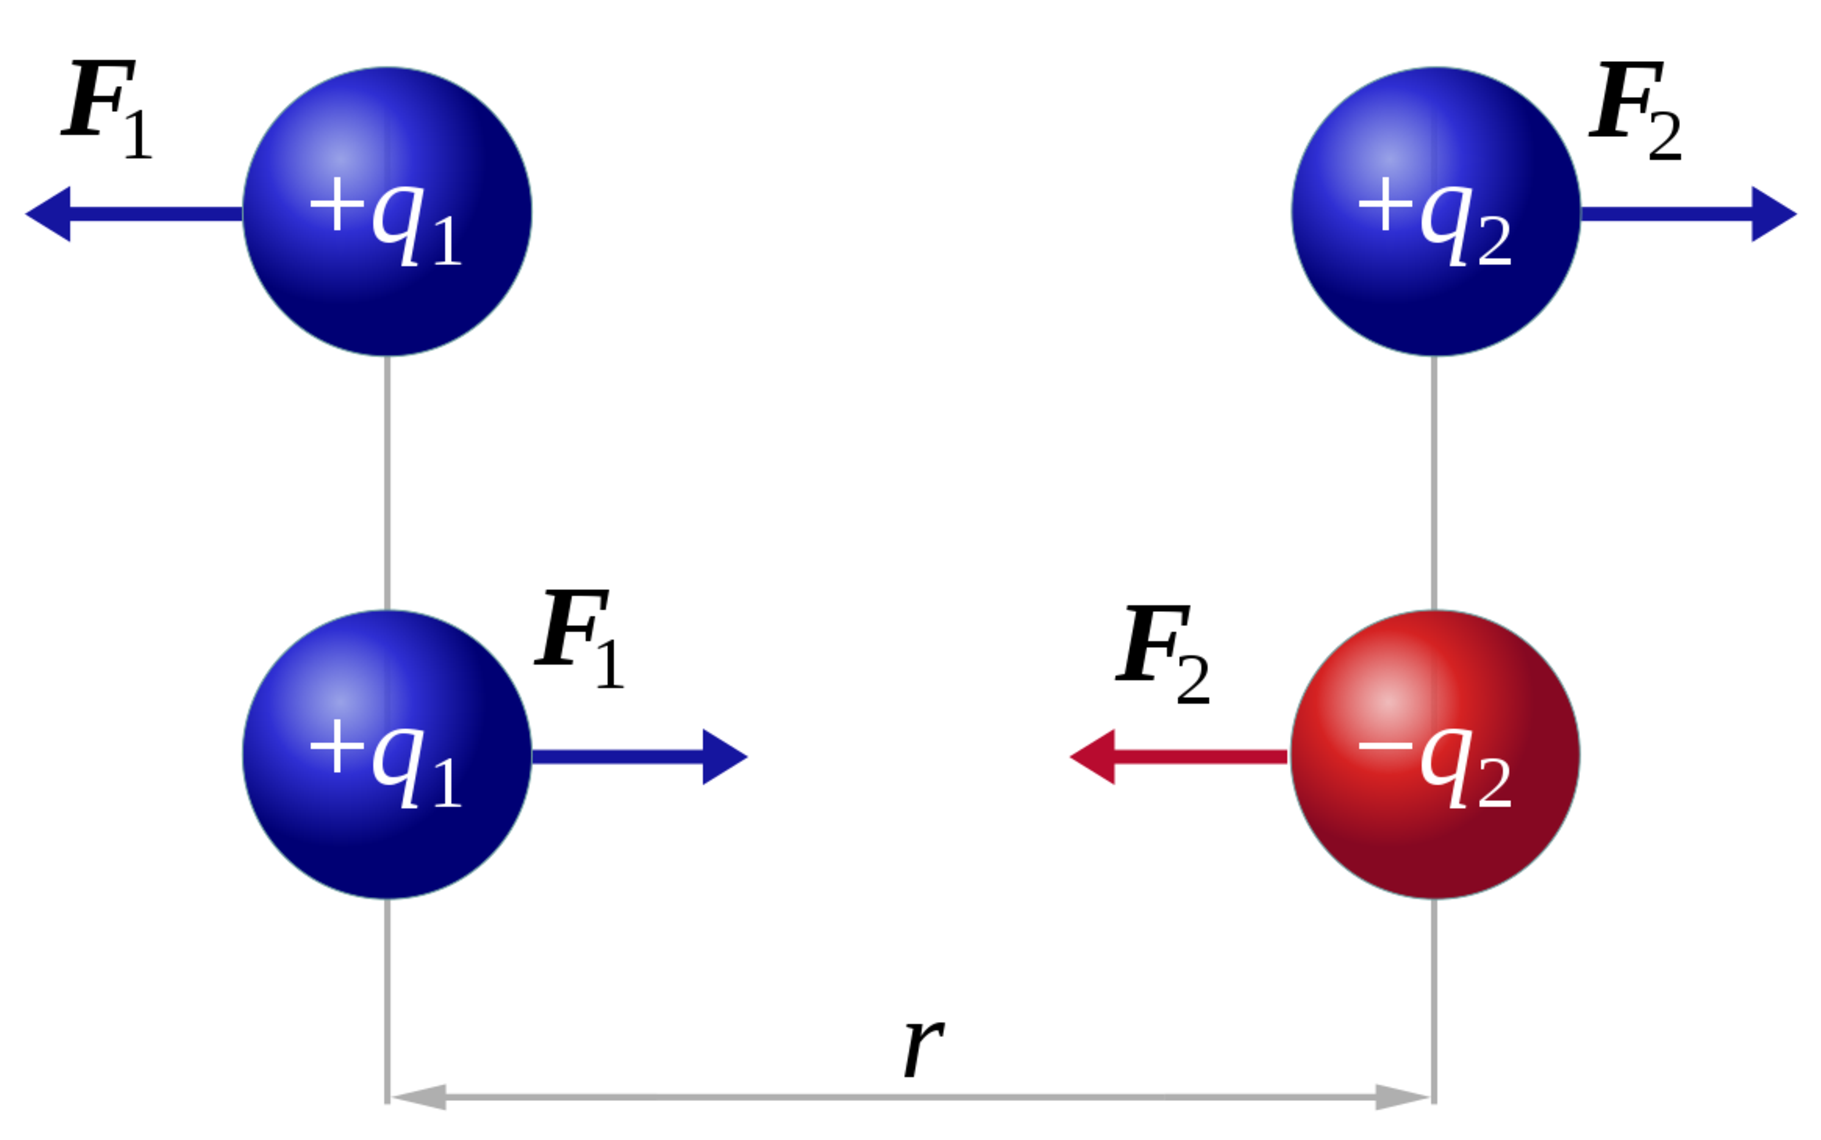
\includegraphics[width=0.5\textwidth]{Elektro/Figurer/Coulomb.eps}
    \caption{Diagram af kræfterne på to ladede partikler når deres ladninger har samme eller modsat fortegn. Kilde: \cite{CoulombLawWikipedia2019}.}
    \label{fig:Coulomb}
\end{figure}

Coulombkraften overholder også princippet om \emph{superposition}: Hvis to ladninger $q_2$ og $q_3$ begge påvirker en ladning $q_1$, så kan den samlede kraft på $q_1$ skrives som en sum, $\va{F}_\text{Total}=\va{F}_{12}+\va{F}_{13}$. Selv for et arbitrært antal ladninger $q_i$, hvor $i=2,3,\dots,N$, der påvirker $q_1$, kan kraften skrives som
\begin{equation} \label{elma:eq:superpos}
    \va{F}=\frac{q_1}{4\pi\varepsilon_0}\sum_{i=2}^{N}\frac{q_i}{\abs{\va{r}_{1i}}^3}\va{r}_{1i} \, .
\end{equation}

Sammenlignet med de kræfter vi typisk arbejder med i mekanik, er Coulombkraften meget speciel på den måde, at den vekselvirker på afstand. F.eks. er friktionskraften og normalkraften kun relevante, når to legemer er i fysisk kontakt. Men Coulombkraften kan skubbe eller tiltrække, om to ladninger er i kontakt, en meter adskilt, eller i modsatte ender af Mælkevejen!
Forestil dig nu følgende hypotetiske scenarie: To ladninger $q_1=\SI{e11}{\coulomb}$ og $q_2=\SI{-e11}{\coulomb}$\footnote{Bemærk at disse ladninger er meget store. Ladningen på én elektron er $\sim\SI{1.6e-19}{\coulomb}$, så det er nærmest umuligt at akkumulere sådan en stor ladning på et sted.}, hver med masse $\SI{1}{\kilogram}$, bliver produceret på samme tid, og placeret præcis et lysår, eller \SI{9.46e15}{\meter}, fra hinanden. Coulombkraften der påvirker de to er så
\begin{equation}
    F=\frac{1}{4\pi\epsilon_0}\frac{\left(\SI{e11}{\coulomb}\right)\times\left(\SI{-e11}{\coulomb}\right)}{\left(\SI{9.46e15}{\meter}\right)^2}=\SI{-1.00}{\newton} \, .
\end{equation}
Hver ladning vil altså føle en tiltrækkende kraft på \SI{1}{\newton} og begynde at accelerere med \SI{1}{\meter\per\second\squared}.

\section{Elektriske felter}
Ovenstående konklusion ledte historisk set til motivationen for, at implementere hvad vi i dag kalder det \emph{elektriske felt}. Et felt skal forstås som noget der eksisterer alle vegne, og der kan sendes signaler igennem dette -- ligesom bølger på en vandoverflade. I feltbeskrivelse tiltrækkes to ladninger via Coulombkraften, fordi feltet fra den ene ladning så at sige fortæller den anden ladningen, at den gerne vil hen imod eller væk fra den første ladning. Ladningen $q_1$ påvirker altså det elektriske felt, som ladningen $q_2$ oplever. Derfra påvirker feltet $q_2$, hvilket resulterer i en tiltrækning eller frastødning. Samme proces sker i modsat retning. Feltet påvirkes af $q_2$, som så påvirker $q_1$. Det elektriske felt er altså et ``medie'', som bliver påvirket af, og som påvirker ladninger.

Det elektriske felt ved en position $\va{r}$, der dannes af ladningen $q$ i punktet $\va r_0$, defineres til at være
\begin{equation} \label{eq:e-felt_punktpartikel}
    \va{E}=\frac{1}{4\pi\varepsilon_0}\frac{q}{\abs{\va r - \va r_0}^3}(\va r - \va r_0) \, .
\end{equation}
Med andre ord, hvis vi vil beregne det elektriske felt fra en ladning $q_1$, som påvirker en anden ladning $q_2$, ligesom på figur \ref{fig:Coulomb}, får vi relationen
\begin{equation} \label{eq:kraft_fra_e-felt}
    \va{E}_{12}=\frac{1}{4\pi\varepsilon_0}\frac{q_1}{\abs{\va r_2 - \va r_1}^3}(\va r_2 - \va r_1)=\frac{\va{F}_{12}}{q_2} \, .
\end{equation}
%
Helt generelt opfylder det elektriske felt, at kraften på en ladning $q$, som resultat af alle elektriske vekselvirkninger er
%
\begin{align} \label{eq:e-felt_def}
    \va F = q\va E \, ,
\end{align}
hvor $\va{E}$ er det totale elektriske felt, der påvirker $q$.

\subsection{Elektriske feltlinjer}

I princippet er vi færdige med elektrostatik, hvilket er studiet af, hvordan ladninger i hvile påvirker hinanden. Ud fra superpositionsprincippet, ligning \eqref{elma:eq:superpos}, kan vi bestemme det elektriske felt af et vilkårligt system af ladninger, og relationen mellem $\va{E}$ og $\va{F}$ fortæller os, hvordan det påvirker andre ladninger.

Meget af det arbejde man vil blive udsat for i elektrostatik ligger dog i at bestemme feltet. Hvad nu hvis feltet ikke var dannet af et endeligt antal punktpartikler med veldefineret ladning, men i stedet var dannet af en kontinuert ladningsfordeling i en given form\footnote{Et eksempel kunne være en skive, hvor skivens overflade har en bestemt mængde ladning per areal.}? Da kan man ikke bruge superpositionsprincippet på formen i ligning \eqref{elma:eq:superpos}, men man må bruge en generaliseret version, som er defineret i form af et integrale i stedet for en sum. Dette gør dog tingene en hel del mere besværlige at arbejde med. Derfor bliver det enormt vigtigt at kunne visualisere og skabe en intuition for de elektriske felter, hvilket kan opnås ved at tegne dets \emph{feltlinjer}. Disse er linjer, der indikerer både retning og styrke af et felt. Retningen af feltet er det samme, som den retning en positiv ladning ville blive skubbet i, hvis den blev placeret i feltet.

Når man tegner de elektriske feltlinjer om en punktladning, kan det repræsenteres som pile, der peger enten ind imod eller ud fra partiklen afhængig af ladningen, som vist på figur \ref{fig:pointcharges}.
\begin{figure}[h!]
    \centering
    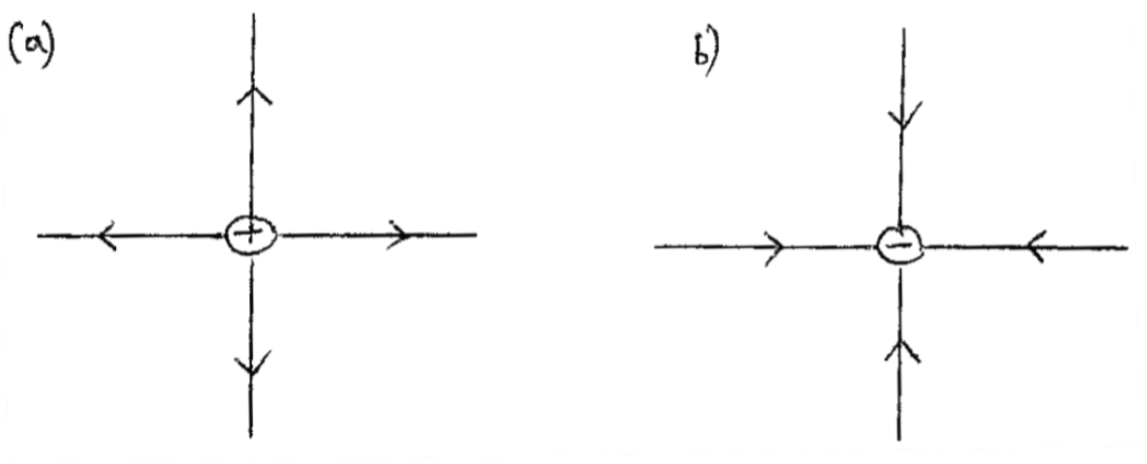
\includegraphics[width=0.8\textwidth]{Elektro/Figurer/fieldline_pointcharges.PNG}
    \caption{Elektriske feltlinjer om en (a) positiv punktladning og en (b) negativ punktladning.}
    \label{fig:pointcharges}
\end{figure}

\noindent Desto flere linjer der er tegnet, jo stærkere er feltet, se figur \ref{fig:pointchargesstrong}. 
\begin{figure}[h!]
    \centering
    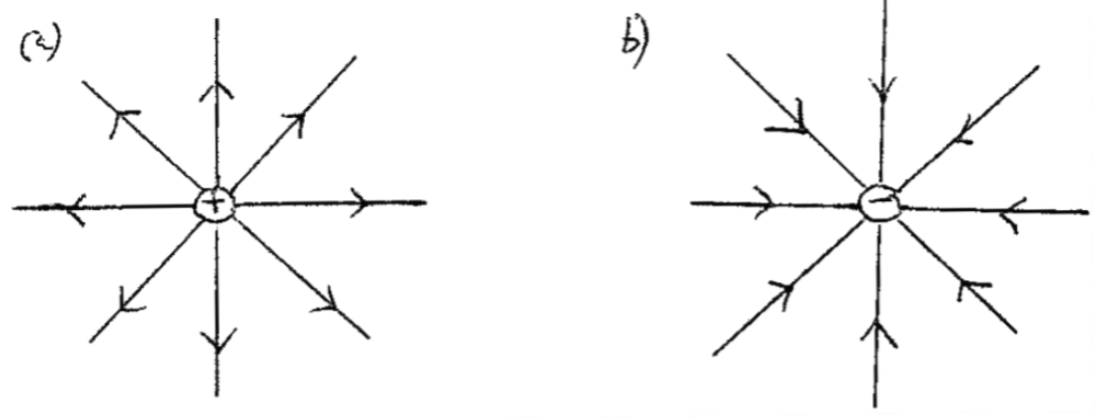
\includegraphics[width=0.8\textwidth]{Elektro/Figurer/fieldline_pointcharges2.PNG}
    \caption{Elektriske feltlinjer om en (a) positiv punktladning og en (b) negativ punktladning med dobbelt så store ladninger som på figur \ref{fig:pointcharges}.}
    \label{fig:pointchargesstrong}
\end{figure}
Som et sidste eksempel kan vi også tegne feltlinjerne for par af punktladninger med enten samme eller forskellig ladning, figur \ref{fig:ElectricFieldLinesTwoCharges}.
\begin{figure}[h!]
    \centering
    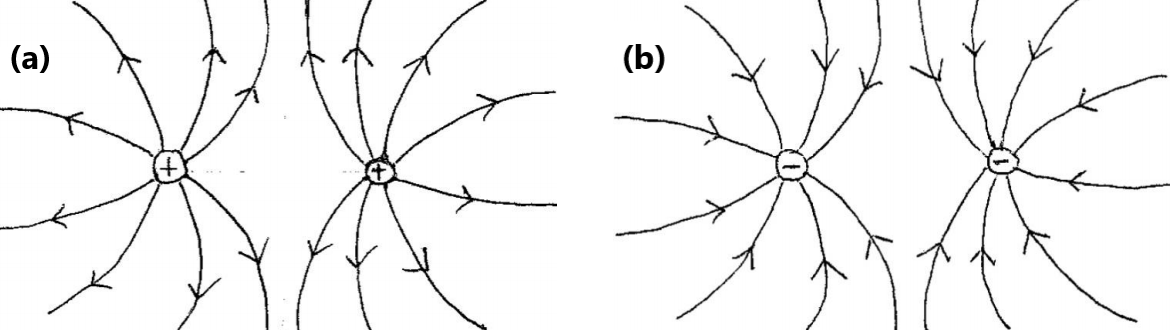
\includegraphics[width=\textwidth]{Elektro/Figurer/fieldline_twocharges.PNG}
    \newline
    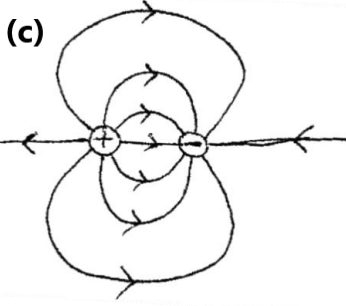
\includegraphics[width=0.37\textwidth]{Elektro/Figurer/fieldline_twocharges2.PNG}
    \caption{Elektriske feltlinjer om par af punktladninger af samme størrelse, (a) for to positive ladninger, (b) to negative ladninger, (c) to modsatte ladninger.}
    \label{fig:ElectricFieldLinesTwoCharges}
\end{figure}
Med disse eksempler i mente, kan vi skrive et sæt regler og yderligere kommentarer om feltlinjer. Nogle stammer fra ren intuition, mens andre følger fra mere avanceret fysik. De er ikke i nogen specifik rækkefølge; det kan endda diskuteres, om de er lige vigtige.
\begin{enumerate}
    \item Feltlinjer eksisterer ikke i virkeligheden. Det er blot en visuel repræsentation som hjælper os med at fortolke fysikken.
    \item Linjernes retning er samme retning som kraften på en positiv ladning i det elektriske felt.
    \item Ovenstående figurer er todimensionelle repræsentationer. I virkeligheden eksisterer felter i 3 dimensioner, men ofte er den todimensionelle repræsentation nok til, at fremhæve den fysik vi er interesserede i.
    \item Feltets tæthed er antallet af feltlinjer per areal (eller volumen i 3D). Feltets tæthed er direkte proportionalt med feltstyrken, så hvis tætheden af feltlinjer fordobles, da vil feltstyrken også fordobles.
    \item Antallet af feltlinjer på en tegning er arbitrær! Hvad der er vigtigt, er den relative tæthed fra et sted til et andet på tegningen.
    \item Hvis der ikke er nogen feltlinje i et område, betyder det at feltstyrken er nul? Ikke nødvendigvis! Det er op til fysikeren, at gøre det nemt at fortolke, hvorhenne feltet faktisk er nul, og hvad der bare er ``mellem linjerne''.
    \item Et eksempel på hvor feltstyrken er nul, er midtpunktet mellem to ladninger af samme størrelse og fortegn. Det er nyttigt at indikere på sit diagram, hvor dette punkt er.
    \item Feltlinjer må aldrig røre hinanden. Dette ville indikere et uendeligt stærkt felt, hvilket ikke er fysisk muligt!
    \item Feltlinjer må aldrig krydse hinanden. Udover en uendelig feltstyrke, ville det betyde forskellige feltretninger i samme punkt.
    \item Elektrostatiske felter starter altid på positive ladninger og slutter på negative.
    \item Feltlinjer viser ikke nødvendigvis den ``sti'', en positiv ladning ville bevæge sig gennem feltet. Det indikerer kun retningen af kraften, ladningen bliver påvirket med.
\end{enumerate}

\section{Elektrisk flux} \label{sec:elektrisk_flux}

I dette og de følgende afsnit vil vi introducere konceptet elektrisk flux, hvilket spiller en stor rolle i elektrostatik. Specielt er den elektriske flux et helt central begreb ift. at formulere Gauss lov, som vi vil kigge på i senere i afsnit \ref{sec:gauss}. Før vi kigger på den præcise definition af elektrisk flux, er det dog værd først at kigge på en sammenhæng mellem feltlinjer og ladning, som vi ikke har dækket endnu.

Vi betragter en kasse, som indeholder en mængde ladning. Da man kan se, at hvis der er tale om en positiv ladning, som på figur \ref{fig:ElectricFluxVisualisation}a,b, vil de elektriske feltlinjer gå ud af kassen. Man siger da, at der er en flux af feltlinjer ud igennem kassens sider. Havde vi i stedet kigget på en negativ ladning, som på figur \ref{fig:ElectricFluxVisualisation}c,d, ville feltlinjerne gå ind i kassen. Man siger da, at der er en flux af feltlinjer ind igennem kassens sider. Ud fra vores viden om elektriske feltlinjer så ved vi, at fordobler vi ladningen, så vil antallet af feltlinjer fra denne ladning også fordobles. Dette er præcis, hvad vi ser fra figur \ref{fig:ElectricFluxVisualisation}a til figur \ref{fig:ElectricFluxVisualisation}b og fra figur \ref{fig:ElectricFluxVisualisation}c til figur \ref{fig:ElectricFluxVisualisation}d.

\begin{figure}[h!]
    \centering
    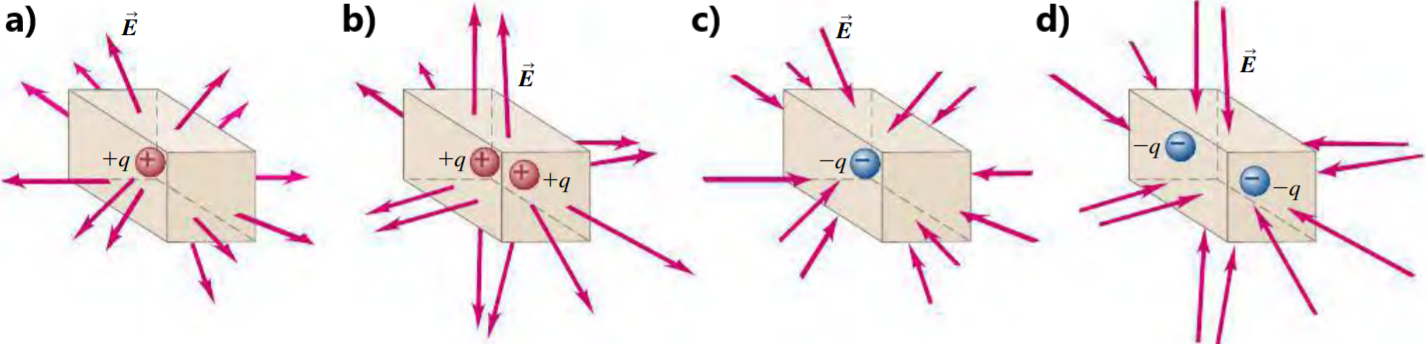
\includegraphics[width=\textwidth]{Elektro/Figurer/ElektricFluxVisualisation.PNG}
    \caption{a) En enkelt positiv ladning i en kasse giver anledning til en udadrettet flux af feltlinjer. b) To positive ladninger giver anledning til dobbelt så stor flux som i (a) gennem den samme kasse, da ladningen er dobbelt så stor. c) En enkelt negativ ladning i en kasse giver anledning til en indadrettet flux af feltlinjer med samme antal feltlinjer som i (a) gennem den sammme kasse. c) To negative ladninger giver anledning til dobbelt så stor flux som i (c) gennem den samme kasse, da ladningen er dobbelt så stor. Kilde: figur 22.2 i \cite{youngSearsZemanskyUniversity2016}.}
    \label{fig:ElectricFluxVisualisation}
\end{figure}

Betragter vi nu den samme kasse, denne gang uden nogen ladning, figur \ref{fig:ElectricFluxVisualisationBoxWithoutCharge}a, så vil der ikke være noget, som kan skabe elektriske feltlinjer, og der vil altså ikke være nogen flux af feltlinjer gennem kassens sider. Indsætter vi i stedet to partikler med ladningerne $q$ og $-q$ i kassen, så vil disse begge skabe elektriske feltlinjer. Det må dog gælde, da de to ladninger har den samme størrelse, at antallet af feltlinjer fra den positive ladning, der vil gå ud igennem kassens sider, er det samme som antallet af feltlinjer fra den negative ladning, der vil gå ind igennem kassens sider, se figur \ref{fig:ElectricFluxVisualisationBoxWithoutCharge}b. Vi kan således konkludere, at den totale flux af feltlinjer gennem kassens sider må være $0$, da feltlinjerne ud og ind af kassen udligner hinanden.  

\begin{figure}[h!]
    \centering
    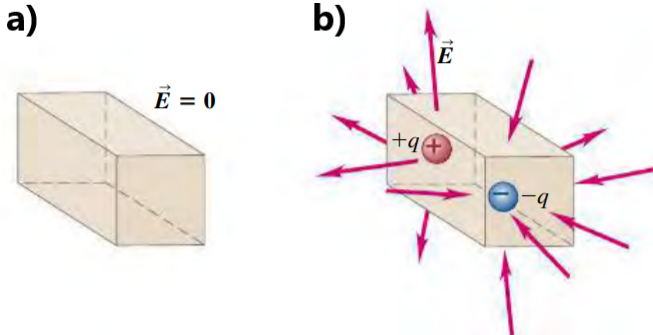
\includegraphics[width=.5\textwidth]{Elektro/Figurer/ElektricFluxVisualisation2.PNG}
    \caption{a) En kasse uden ladning vil ikke have en flux af feltlinjer. b) Den totale ladningen for to partikler med ladningerne $q$ og $-q$ vil være $0$, hvorfor denne konfiguration ikke vil have en flux af feltlinjer. Dette kan også ses af, at fluxen af feltlinjer fra hver af ladningerne udligner hinanden. Kilde: figur 22.3 i \cite{youngSearsZemanskyUniversity2016}.}
    \label{fig:ElectricFluxVisualisationBoxWithoutCharge}
\end{figure}

\subsection{Elektrisk flux i uniformt elektrisk felt}

Ses der først på et uniformt elektrisk felt, altså et elektrisk felt hvor styrken og retningen altid er den samme, så vil den elektriske flux, $\Phi_E$, gennem et areal $A$, der er fladt og står vinkelret på de elektriske feltlinjer, figur \ref{fig:ElectricFlux1}, være givet ved
\begin{align} \label{eq:ElectricFluxUniformFieldFlatPerpendicularArea}
	\Phi_E &= EA \, ,
\end{align}
hvor $E$ er styrken af det elektriske felt, som giver anledning til de elektriske feltlinjer. Heraf kan det ses for uniforme elektriske felter, at den elektriske flux er direkte proportionel med både styrken af det elektriske felt, $E$, samt med størrelsen af arealet, $A$. Det betyder, at hvis arealet øges, så vil den elektriske flux også øges med samme faktor, og ligeså for styrken af feltet.
\begin{figure}[h!]
    \centering
    \begin{subfigure}[t]{.3\textwidth}
        \centering
        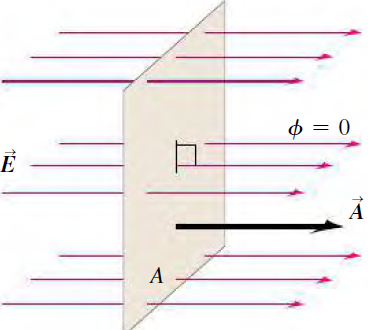
\includegraphics[width=\columnwidth]{Elektro/Figurer/ElectricFlux1.PNG}
        \caption{Overfladen står vinkelret på det elektriske felt, så $\va{E}$ og $\va{A}$ er parallelle (vinklen mellem $\va{E}$ og $\va{A}$ er $\phi = \SI{0}{\degree}$). Fluxen bliver derved $\Phi_E = \va{E} \cdot \va{A} = EA$.}
        \label{fig:ElectricFlux1}
    \end{subfigure}
    \hfill
    \begin{subfigure}[t]{.3\textwidth}
        \centering
        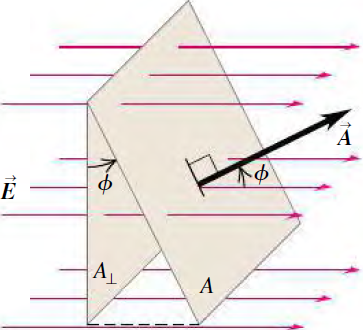
\includegraphics[width=\columnwidth]{Elektro/Figurer/ElectricFlux2.PNG}
        \caption{Overfladen er vinklet med vinklen $\phi$ fra at stå vinkelret på det elektriske felt, så vinklen mellem $\va{E}$ og $\va{A}$ er $\phi$, hvorved fluxen bliver $\Phi_E = \va{E} \cdot \va{A} = EA\cos(\phi)$.}
        \label{fig:ElectricFlux2}
    \end{subfigure}
    \hfill
    \begin{subfigure}[t]{.3\textwidth}
        \centering
        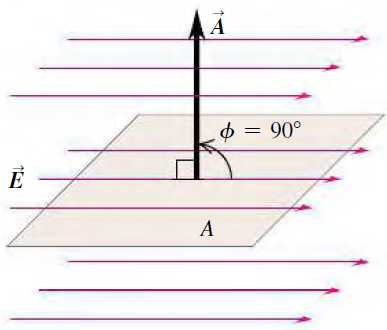
\includegraphics[width=\columnwidth]{Elektro/Figurer/ElectricFlux3.PNG}
        \caption{Overfladen vinklet således, at den er parallel til det elektriske felt, så $\va{E}$ og $\va{A}$ står vinkelret på hinanden (vinklen mellem $\va{E}$ og $\va{A}$ er $\phi = \SI{90}{\degree}$). Fluxen bliver derved $\Phi_E = \va{E} \cdot \va{A} = EA\cos(\SI{90}{\degree}) = 0$.}
        \label{fig:ElectricFlux3}
    \end{subfigure}
    \caption{En flad overflade i et uniformt elektrisk felt. Den elektrisk flux $\Phi_E$ gennem overfladen er givet ved prikproduktet mellem det elektriske felt $\va{E}$ og arealvektoren $\va{A}$. Kilde: figur 22.6 i \cite{youngSearsZemanskyUniversity2016}.}
    \label{fig:ElectricFlux}
\end{figure}

Vinkles dette areal nu således, at det ikke længere står vinkelret på de elektriske feltlinjer, da vil færre af disse passere gennem arealet, idet feltlinjerne kun passerer gennem den del af arealet, $A_\perp$, som står vinkelret på dem, hvilket på figur \ref{fig:ElectricFlux2} og \ref{fig:ElectricFlux3} er svarende til $A_\perp = A\cos(\phi)$ per trigonometri.
Ligning \eqref{eq:ElectricFluxUniformFieldFlatPerpendicularArea} generaliseres derved til
\begin{align} \label{eq:ElectricFluxUniformFieldFlatArea}
	\Phi_E &= EA\cos(\phi) \, .
\end{align}
Dette kan identificeres som værende prikproduktet mellem $\va{E}$ og $\va{A}$ (se evt. ligning \eqref{mat:prikprodukt} ift. prikproduktet)
\begin{align} \label{eq:ElectricFluxUniformFieldFlatAreaScalarProduct}
	\Phi_E &= \va{E} \cdot \va{A} \, ,
\end{align}
hvor $\va{A}$ er \emph{arealvektoren}, hvis retning er repræsenteret ved en enhedsvektor $\vu{n}$ (``normalvektoren''), der står vinkelret på arealet, og hvis længde er lig med størrelsen af arealet, se figur \ref{fig:ElectricFlux}. Vi kan altså arealvektoren som
\begin{align} \label{eq:ElectricFluxAreaVector}
	\va{A} &= A\vu{n} \, .
\end{align}
Idet at en overflade altid har to sider, da vil der være mulighed for to retninger af normalvektoren, og dermed også for arealvektoren, hvorfor dennes retning altid skal specificeres. Ofte betragter vi fluxen, hvilken f.eks. kan stamme fra en punktladning, ud gennem et lukket overflade, og i disse tilfælde vælger vi per konvention normalvektorens retning til at være udad fra overfladen. Det vil dermed være retningen af det elektriske felt, der bestemmer om den elektriske flux er positiv eller negativ. Fra ligning \eqref{eq:ElectricFluxUniformFieldFlatAreaScalarProduct} kan man se, at $\Phi_E>0$, når det elektriske felt peger ud igennem den lukkede overflade, da vinklen $\phi$ mellem feltet og arealvektoren her vil opfylde at: $0\degree < \phi < 90\degree$. Modsat vil man have, at $\Phi_E < 0$, når det elektriske felt peger ind igennem den lukkede overflade, hvilket følger af et lignede argument som ovenfor.

\subsection{Generalisering af elektrisk flux}

I foregående afsnit blev der fundet en beskrivelse af den elektriske flux for et uniformt elektrisk felt gennem en flad overflade, men dette er ikke altid tilfældet. Man kan forestille sig, at det elektriske felt ikke er uniformt, altså at det ændrer sig alt efter ens rummelige placering, eller at overfladen, som man regner fluxen gennem, er krum, som f.eks. en kugleskal, hvilket vi endnu ikke har taget højde for. Vi vil derfor generalisere udtrykket for den elektriske flux fundet i ligning \eqref{eq:ElectricFluxUniformFieldFlatAreaScalarProduct}.

Til dette formål opdeler vi dermed overfladen i mange små dele $\dd{A}$, som hver har sin egen normalvektor $\vu{n}$ vinkelret på dem, har en arealvektor $\dd{\va{A}} = \dd{A}\vu{n}$, og kan ses som værende i et uniformt elektriske felt\footnote{Ethvert elektrisk felt vil være uniformt, hvis man kigger på det indefor en tilpas lille volumen. Dette er lidt det samme, som at jorden for os opleves som værende flad, selvom den jo i det store billede er rund.}. Den elektriske flux gennem hvert af disse arealer beregnes ved ligning \eqref{eq:ElectricFluxUniformFieldFlatAreaScalarProduct}, og resultaterne integreres op (husk at integraler en form for ``sum'') for at finde den totale elektriske flux
\begin{align} \label{eq:ElectricFlux}
	\Phi_E &= \int_S \va{E} \cdot \dd{\va{A}} \, .
\end{align}
Integralet i ligning \eqref{eq:ElectricFlux} er et overfladeintegral (dobbeltintegral), hvor $S$ angiver den overflade, som man integrerer over.

\subsubsection{Elektrisk flux gennem en cirkulær overflade}

\begin{figure}[t]
    \centering
    \begin{subfigure}[t]{.45\textwidth}
        \centering
        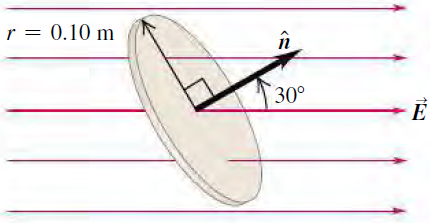
\includegraphics[width=\columnwidth]{Elektro/Figurer/ElectricFluxThroughADisk.PNG}
        \caption{En circulær disk med radius $R = \SI{0.10}{\meter}$ er placeret i et uniformt elektrisk felt $\va{E}$, så dens normalvektor $\vu{n}$ er i en vinkel af $\phi = \SI{30}{\degree}$ til det elektriske felt. Kilde: figur 22.7 i \cite{youngSearsZemanskyUniversity2016}.}
        \label{fig:ElectricFluxThrougADisk}
    \end{subfigure}
    \hfill
    \begin{subfigure}[t]{.45\textwidth}
        \centering
        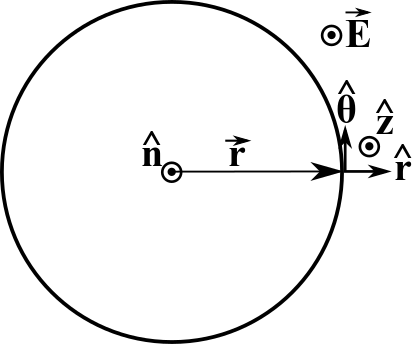
\includegraphics[width=.65\columnwidth]{Elektro/Figurer/ElectricFluxExercise.png}
        \caption{Den samme cirkulære disk placeres nu i et ikke uniformt elektrisk felt $\va{E} = E_0 r \vu{z}$ i samme retning som det foregående, hvor $E_0 = \SI{2.0e3}{\newton/\coulomb}$, og disken rettes nu op således, at den står vinkelret på feltet ($\phi = 0$).}
        \label{fig:ElectricFluxThrougADisk2}
    \end{subfigure}
    \caption{En cirkulær disk med radius $R = \SI{0.10}{\meter}$ placeres i et elektrisk felt $\va{E}$.}
    \label{fig:ElectrixFluxExample}
\end{figure}

Som eksempel kan vi se på en rund disk placeret i et uniformt elektrisk felt $\va{E}$ med størrelsen $\SI{2.0e3}{\newton/\coulomb}$. Disken har en radius på $R = \SI{0.10}{\meter}$ og er vinklet i forhold til det elektriske felt med vinklen $\phi = \SI{30}{\degree}$. Diskens normalvektor er orienteret som set på figur \ref{fig:ElectricFluxThrougADisk}, hvilket er nødvendigt at specificere, da en disk ikke er en lukket overflade og dermed ikke har en inderside og en yderside. Vi ønsker nu at finde den elektriske flux gennem disken.

Idet disken er placeret i et uniformt elektrisk felt benytter vi ligning \eqref{eq:ElectricFluxUniformFieldFlatAreaScalarProduct}
\begin{align}
    \Phi_E &= \va{E} \cdot \va{A} \, .
\end{align}
Vi skal altså kende det elektriske felt $\va{E}$ og arealvektoren $\va{A}$. Styrken af det elektriske felt er som nævnt givet til at være $E = \SI{2.0e3}{\newton/\coulomb}$. Arealvektoren findes ved ligning \eqref{eq:ElectricFluxAreaVector} som arealet af disken ganget med normalvektoren $\vu{n}$, så $\va{A} = A\vu{n}$, hvor $A = \pi R^2$. Vinklen mellem det elektriske felt $\va{E}$ og arealvektoren $\va{A}$ er $\phi = \SI{30}{\degree}$, så vi får fluxen gennem disken til at være
\begin{align}
    \Phi_E &= EA\cos(\phi)
        = E \pi R^2 \cos(\phi)
        = \left(\SI{2.0e3}{\frac{\newton}{\coulomb}}\right) \left(\SI{0.0314}{\meter^2}\right) \cos\left(\SI{30}{\degree}\right)
        = \SI{54}{\frac{\newton\meter^2}{\coulomb}} \, .
\end{align}
Placeres den samme disk nu i et ikke uniformt elektrisk felt, $\va{E} = E_0 r \vu{z}$, hvor $E_0 = \SI{2.0e3}{\newton/\coulomb}$, som set på figur \ref{fig:ElectricFluxThrougADisk2}, kan ligning \eqref{eq:ElectricFluxUniformFieldFlatAreaScalarProduct} ikke længere bruges til at beregne fluxen, men man skal i stedet benytte ligning \eqref{eq:ElectricFlux}. Idet at det elektriske felt kun afhænger af afstanden til centrum, $r$, og da disken er symmetrisk omkring origo (centrum af disken), kan man skrive arealetelementet $\dd{A}$ ved brug af ligning \eqref{eq:ArealElementMat}. Det giver at
\begin{align}
    \dd{\va{A}} &= 2\pi r \dd{r} \vu{n} = 2\pi r \dd{r} \zhat \, ,
\end{align}
hvor det er brugt, at $\vu{n} = \zhat$ her, som det fremgår af figur \ref{fig:ElectricFluxThrougADisk2}. Fluxen gennem hele disken findes dermed vha. \eqref{mat:eq:polardoubleint}, hvilket giver
\begin{align} \label{eq:ElectricFluxExampleStep1}
	\Phi_E &= \int_S \va{E} \cdot \dd{\va{A}}
	    = \int_{0}^{R} \left(E_0 r \vu{z}\right) \cdot \left(2\pi r \dd{r} \zhat \right)
	    = 2\pi E_0 \int_{0}^{R} r^2 \left(\zhat \cdot \zhat)\right \dd{r}
	    = 2\pi E_0 \int_{0}^{R} r^2 \dd{r} \, ,
\end{align}
hvor det er benyttet, at $\zhat \cdot \zhat = 1$, og at man må sætte konstanter udenfor integralet. Udregnes dette integral fås
\begin{align} \label{eq:ElectricFluxExampleStep2}
	\Phi_E &= 2\pi E_0 \int_{0}^{R} r^2 \dd{r}
	    = 2\pi E_0 \left[\frac{1}{3}r^3\right]_{0}^{R}
	    = \frac{2}{3}\pi E_0 \left[ r^3\right]_{0}^{R}
	    = \frac{2}{3} \pi E_0 R^3 \, ,
\end{align}
hvor leddet tilhørende den nedre grænse er droppet, da det giver nul her. Indsættes den givne værdi for det elektriske felts styrke $E_0 = \SI{2.0e3}{\newton/\coulomb}$ samt diskens radius $R = \SI{0.10}{\meter}$ fås fluxen gennen disken til at være
\begin{align}
    \Phi_E &= \frac{2}{3} \pi \cdot \SI{2.0e3}{\frac{\newton}{\coulomb}} \cdot (\SI{0.10}{\meter})^3
	    = \SI{4.2}{\frac{\newton\meter^2}{\coulomb}} \, .
\end{align}


\subsection{Gauss' lov} \label{sec:gauss}
Gauss' lov er en måde at beskrive forholdet mellem elektriske ladninger og felter. Loven fortæller, at den elektriske flux gennem en lukket overflade, som indelukker et endeligt volumen, er proportional med den totale elektriske ladning indenfor overfladen.

Dette kan vi vise ved først at kigge på en enkelt positivt ladet partikel med ladning $q$. Denne ladningen placeres i centrum af en imaginær sfære med radius $R$, hvor vi så vil regne fluxen gennem denne sfæres overflade. Fra ligning \eqref{eq:e-felt_punktpartikel} vides det, at det elektriske felt fra ladningen er
\begin{align}
    \va{E} = \frac{1}{4\pi\epsilon_0} \frac{q}{\abs{\va{r}}^3} \va{r} \, ,
\end{align}
da udgangspunktet $\va{r}_0$ her er i sfærens centrum, så $\va{r}_0$ er nulvektoren her. Ved ethvert punkt på overfladen af sfæren vil det elektriske felt (som peger udad) være vinkelret til overfladen, da feltlinjerne fra ladning udsendes ligeligt i alle retninger, som på figur \ref{fig:pointchargesstrong}. Da må styrken af det elektriske felt, $E$, her  kun afhænger af afstanden til centrum, $r$, må feltet altså have samme styrke på hele sfærens overfalde. Derved bliver den totale elektriske flux blot produktet af det elektriske felts styrke på overfladen af sfæren (radius $R$) og overfladearealet af sfæren selv $A$. Altså får man at
\begin{align} \label{eq:GaussLawSphere}
    \Phi_E &= EA = \frac{1}{4\pi\epsilon_0} \frac{q}{R^2} (4 \pi R^2) = \frac{q}{\epsilon_0} \, .
\end{align}
Fluxen er derved uafhængig af sfærens radius og afhænger kun af den indesluttede ladning $q$. Bemærk specielt at fluxen som påstået er proportional med den indesluttede ladning $q$ med $1/\epsilon_0$ som proportionalitetskonstant. 

\begin{figure}[h!]
    \centering
    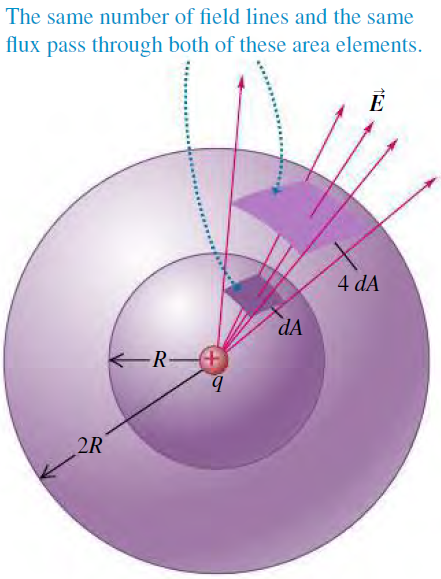
\includegraphics[width=.4\textwidth]{Elektro/Figurer/GaussLawProjectingOntoASphere.PNG}
    \caption{Projektion af et lille areal $\dd{A}$ fra overfladen af en sfære med radius $R$ på overfladen af en sfære med radius $2R$. Kilde: figur 22.11 i \cite{youngSearsZemanskyUniversity2016}.}
    \label{fig:GaussLawProjectingOntoASphere}
\end{figure}

Uafhængiheden af sfærens radius kan også ses, hvis vi kigger på en lille del af overfladen, arealelementet $\dd{A}$, på sfæren med radius $R$. Projiceres\footnote{Delen af arealet projiceres ved at trække linjer fra ladningen i centrum gennem hjørnerne af arealdelen i afstanden $R$ og ende i afstanden $2R$, hvor slutpunkterne kan forbindes til af vise arealet projiceret på sfæren med radius $2R$.} denne på en sfære med radius $2R$, figur \ref{fig:GaussLawProjectingOntoASphere}, så arealet på sfæren med radius $2R$ bliver $4\dd{A}$, da hver side af arealelementet bliver dobbelt så stor. Men siden det elektriske felt er omvendt proportionalt med afstanden kvadreret ($E \propto 1/r^2$) vil størrelsen af dette være $4$ gange mindre i afstanden $2R$ fra centrum, hvorfor disse frontfaktorer ($4$ og $1/4$) vil gå ud, når fluxen beregnes. Altså vil fluxen gennem de to arealer være ens uafhængigt af de pågældende sfærers radius.

\begin{figure}[h!]
    \centering
    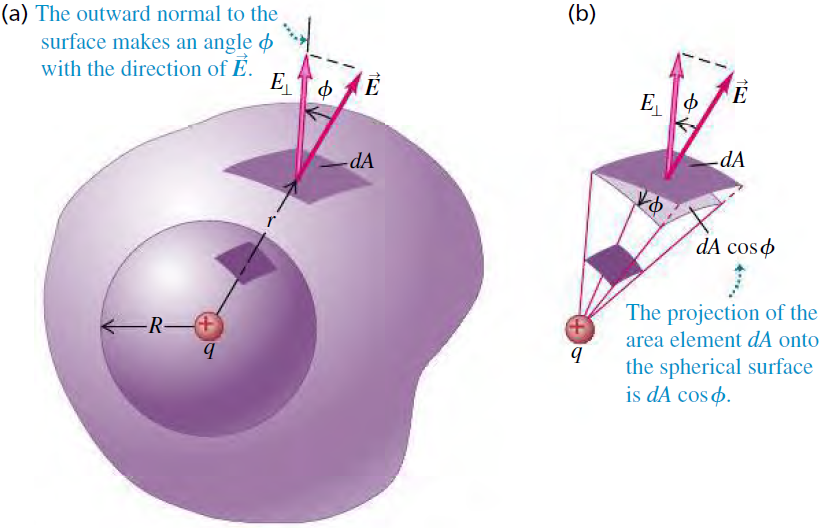
\includegraphics[width=.75\textwidth]{Elektro/Figurer/GaussLawProjectingOntoAnArbitraryShape.PNG}
    \caption{Projektion af et lille areal $\dd{A}$ fra overfladen af en sfære med radius $R$ på overfladen af en ikkesfærisk overflade i afstanden $r$. Kilde: figur 22.12 i \cite{youngSearsZemanskyUniversity2016}.}
    \label{fig:GaussLawProjectingOntoanArbitraryShape}
\end{figure}

For at generalisere Gauss' lov til ikke-sfæriske overflader benyttes projiceringsteknikken igen, men i stedet for en ydre sfære er den indre sfære af radius $R$ omgivet af en irregulær overflade, som på figur \ref{fig:GaussLawProjectingOntoanArbitraryShape}a. Tager vi et lille arealelement $\dd{A}$ på den irregulære overflade i en afstand $r$ til ladningen og projicerer dette ned på en kugleskal i samme afstand, så vil to af siderne, som set på figur \ref{fig:GaussLawProjectingOntoanArbitraryShape}b, blive forkortet med $\cos(\phi)$, hvor $\phi$ er vinklen mellem arealelementets normal $\vu{n}$ og det elektriske felt $\va{E}$. De to resterende sider af arealelementet forbliver uændrede, hvorved det projicerede arealelement er givet ved $\dd{A}\cos(\phi)$. Analogt til at projicere arealelementet, der ikke er vinkelret på det elektriske felt, ned på sfæren, hvor elementet er vinkelret på feltet, da kan man i stedet projicere det elektriske felt, der ikke er vinkelret på arealelementet, på normalvektoren for arealelementet, så denne projektion $E\cos(\phi)$ vil være vinkelret på arealelementet. Dette skyldes, at man uanset hvad får retningen af arealvektoren og det elektriske felt til at være parallelle efter projektion af den ene af dem, hvorved man for at finde fluxen blot multiplicerer den ene med den anden, hvorfor det er irrelevant, om $\cos(\phi)$ er ganget på den ene eller den anden parameter. Den elektriske flux gennem det valgte arealelement bliver derved $E\dd{A}\cos(\phi)$.

Opdeles hele den irregulære overflade i små arealelementer kan fluxen gennem hvert af disse regnes som ovenstående og summeres ved integration over hele overfladen. Den totale elektrisk flux gennem den irregulære overflade, givet ved ligning \eqref{eq:ElectricFlux}, skal være den samme som den totale flux gennem en sfære, som set ovenfor, hvilket per ligning \eqref{eq:GaussLawSphere} er lig $q/\epsilon_0$. Derfor vil den totale flux gennem den irregulære overflade være
\begin{align} \label{eq:GaussLawArbitraryShape}
    \Phi_E &= \oint_S \va{E} \cdot \dd{\va{A}} = \frac{q}{\epsilon_0} \: .
\end{align}
Dette er Gauss' lov, hvilken holder for enhver lukket overflade, der indeslutter en ladning $q$. Cirklen på integralet betyder, at integralet altid skal beregnes over en lukket overflade.

I ovenstående udledning var blot placeret en enkelt ladning $q$ indenfor den irregulære overflade, men Gauss' lov kan generaliseres til at indeholde et vilkårligt antal ladninger
\begin{align} \label{eq:GaussLawGeneral}
    \oint_S \va{E} \cdot \dd{\va{A}} &= \frac{Q_{\text{inde}}}{\epsilon_0} \: ,
\end{align}
hvor $Q_{\text{inde}}$ er den totale ladning indesluttes af overfladen, og $\va{E}$ er det totale elektriske felt beregnet ved superpositionsprincippet.

%
\begin{figure}
    \centering
    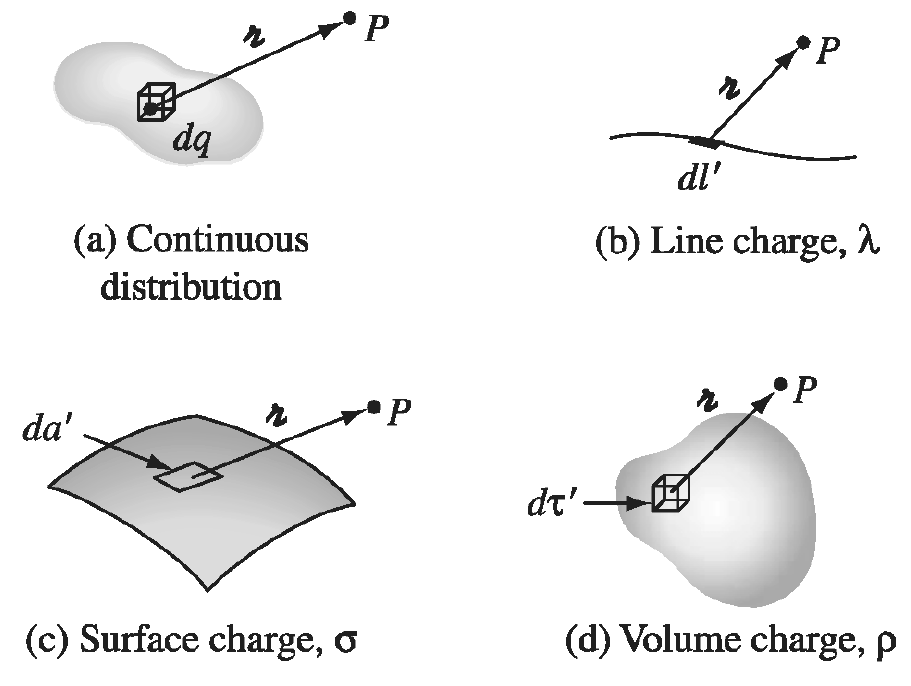
\includegraphics[width=.6\columnwidth]{Elektro/Figurer/ladningsfordeling.PNG}
    \caption{Illustration af kontinuerte ladningsfordelinger i 1, 2 og 3 dimensioner. Det vigtige i figuren er illustrationerne og ikke det vektorer og parametre, der er indtegnet i figuren. Kilde: figur 2.5 i \cite{griffithsIntroductionElectrodynamics2017}.}
    \label{fig:ladningsfordeling}
\end{figure}
%
\subsubsection{Ladningsfordeling}
Så længe et system har en symmetri, der gør det muligt at løse integralet i ligning \eqref{eq:GaussLawGeneral} kan Gauss' lov bruges til at bestemme det elektriske felt overalt i rummet. For at gøre det skal den indesluttede ladning bestemmes. Til at beskrive hvordan ladningen er fordelt i rummet bruges en kontinuert\footnote{For de matematisk interesserede så sikrer kontinuitetskravet at ladningstæthedsfunktionerne er integrable, se side 366 i \cite{stewartCalculusConceptsContexts2006}, således at deres integraler kan bruges til at bestemme mængden af ladning i et område.} \textit{ladningstæthedsfunktion}. At ladningsfordelingen er kontinuert betyder at vi betragter ladning som værende smurt ud i rummet i stedet for at være samlet i diskrete punkter. Ladningstæthedsfunktioner opdeles i tre tilfælde efter hvor mange dimensioner ladningen er fordelt i med hver deres symbol:
%
\begin{itemize}
    \item Lineær ladningstæthed, $\lambda$
    \item Overfladeladningstæthed, $\sigma$
    \item Volumenladningstæthed, $\rho$
\end{itemize}
%
Figur \ref{fig:ladningsfordeling} viser illustrationer af de forskellige typer ladningstætheder. Hvis alt ladningen er samlet på en linje i rummet, så beskrives den ved den lineære ladningstæthed, $\lambda$, uanset hvor krøllet og mystisk denne linje er. Tilsvarende beskriver overfladeladningstætheder, $\sigma$, alt hvad der kan beskrives i to dimensioner, men ikke i én dimension, og i det sidste tilfælde hvor ladningen er fordelt i alle tre rummelige dimensioner bruges volumenladningstætheden, $\rho$. En tæthedsfunktion har den egenskab at dens integral giver mængden af hvad den beskriver indenfor et bestemt område i rummet. På lidt mere almindeligt dansk, så findes ladningen på en linje fra punktet $a$ til punktet $b$, som kaldes $Q_{ab}$, ved at integrere den lineære ladningstæthedsfunktion, $\lambda$:
%
\begin{subequations} \label{eq:ladningsfordeling}
    \begin{align} \label{eq:line_charge}
        Q_{ab} = \int_a^b \lambda \dd{l}.
    \end{align}
    %
    Her er integrationsvariablen $l$, da det gælder generelt for alle linjer. Hvis linjen er ret og i $x$-aksen, så ville integrationsvariablen være $x$. Hvis der er tale om en overfladeladningstæthed, så skal man integrere i to dimensioner. Ladningen i en plan parallelt med $xy$-planen indenfor et rektangel udspændt af punkterne $(x_1,y_1),(x_2,y_1),(x_1,y_2),(x_2,y_2)$ er så
    %
    \begin{align}
        Q = \int \sigma \dd{A} = \int_{x_1}^{x_2}\int_{y_1}^{y_2} \sigma \dd{x}\dd{y}.
    \end{align}
    %
    Er der slutteligt tale om en volumenladningstæthed er der tale om et rummeligt integral
    %
    \begin{align} \label{eq:volumenladning}
        Q = \int \rho \dd{V}.
    \end{align}
\end{subequations}
%
Ofte kan integralerne forsimples ved brug af symmetriargumenter. Et vigtigt specialtilfælde af ligning \eqref{eq:ladningsfordeling} er den uniforme ladningsfordeling. Uniform betyder ensartet eller med andre ord konstant og af ligning \eqref{mat:eq:konstant} fremgår det at konstanter kan trækkes udenfor integralet og således giver ligning \eqref{eq:line_charge}
%
\begin{align}
    Q_{ab} = \int_a^b \lambda \dd{l} = \lambda \int_a^b \dd{l} = \lambda(b-a).
\end{align}
%
At løse disse integraler kan være lidt en kunst og derfor holder vi os her til nogle af de simpleste tilfælde og hjælpe læseren til en introduktion til denne gren af fysikken\footnote{For den interesserede læser så giver \cite{youngSearsZemanskyUniversity2016} en mere uddybende introduktion til emnet, mens \cite{griffithsIntroductionElectrodynamics2017} giver en grundig gennemgang af hele elektrodynamikken.}.

\subsubsection{To uendelig lange ladede cylindere} \label{sec:gauss_lov_eksempel}
Som eksempel på brugen af Gauss' lov kan vi se på to uendelig lange, koaksiale\footnote{De to cylindres ligger begge med centrum langs $\vu{z}$-aksen.} ladede cylindre, hvor den inderste (mørk grå) er en ikkehul cylinder med en uniform volumenladningstæthed $\rho$, mens den ydre (lys grå) er hul og har en uniform overfladeladningstæthed på $\sigma$. Denne opstilling kan ses på figur \ref{fig:GaussLawExample}a. Vi ønsker at bestemme det elektriske felt tre forskellige steder i forhold til cylindrene: Indeni den inderste cylinder (\textcolor{green}{grøn} stiplet linje), mellem den inderste og den yderste cylinder (\textcolor{blue}{blå} stiplet linje) og udenfor den yderste cylinder (\textcolor{red}{rød} stiplet line). For at beregne det elektriske felt disse tre steder indlægges hver sted (altså med radier $r < r_1$, $r_1 < r < r_2$ og $r > r_2$) en Gauss overflade, der her er en Gauss cylinder, da der er cylindrisk symmetri, hvilket skyldes, at det elektriske felt vil blive udsendt i den radiære\footnote{Den radiære retning er langs retningen af $\va{r}$-vektoren. I cylindrisk symmetri vil dette være fra centrum af cylinderen og ud gennem dens sidevægge.} retning $\va{E} = E\vu{r}$. Det bemærkes, at grundet den cylindriske symmetri vil det elektriske felt $\va{E}$ være parallelt med arealvektoren $\dd{\va{A}}$, hvorfor $\va{E} \cdot \dd{\va{A}} = E\dd{A}$. Vi kigger nu på de tre Gauss overflader:

\begin{figure}[t]
    \centering
    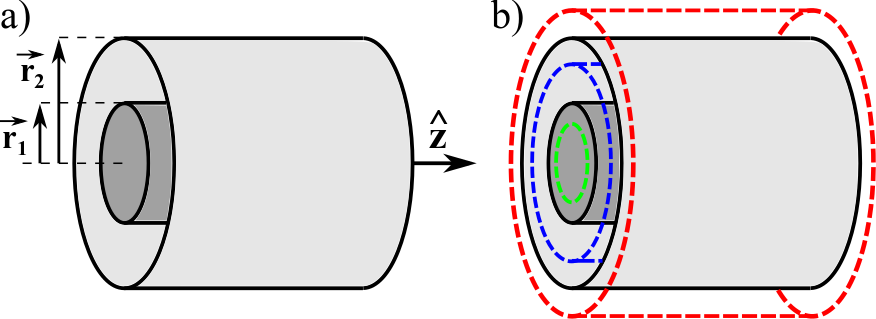
\includegraphics[width=\textwidth]{Elektro/Figurer/GaussLawExample.png}
    \caption{a) En ikkehul cylinder (mørk grå) med radius $r_1$ og uniform volumenladningstæthed $\rho$ per længdeenhed er placeret koaksialt i en hul cylinder (lys grå) med radius $r_2$ og uniform overfladeladningtæthed $\sigma$. Begge cylindre antages at være uendelig lange, således at problemet er cylindrisk symmetrisk over alt. b) Tre Gausscylindre er placeret koaksialt med de to uendeligt lange ladede cylindre: Én indenfor den inderste cylinder, én mellem de to cylindre kun indkapslende den inderste cylinder, og en indkapslende begge cylindre.}
    \label{fig:GaussLawExample}
\end{figure}

\begin{itemize}
    \item $\mathbf{r < r_1}$\textbf{:} Ladningen inden i den inderste cylinder er uniformt fordelt, hvorfor udtrykket for den indesluttede ladning vil være afhængig af cylinderens volumen
    \begin{align}
        Q_{\text{inde}}(r) &= \rho\pi r^2 z \: ,
    \end{align}
    hvor $z$ her angiver en længdeenhed.
    Ved at gøre brug af Gauss' lov (ligning \eqref{eq:GaussLawGeneral}) fås derved
    \begin{align}
        \frac{Q_{\text{inde}}}{\epsilon_0} &= \frac{\rho\pi r^2 z}{\epsilon_0}
            = \oint_S \va{E} \cdot \dd{\va{A}}
            = \oint_S E \dd{A}
            = E \oint_S \dd{A} \: .
    \end{align}
    Idet arealet af en cylinder er givet som produktet af omkredsen af en cirkel og længden af cylinderen fås
    \begin{align}
        \frac{\rho\pi r^2 z}{\epsilon_0} &= E \cdot 2\pi r z \: ,
    \end{align}
    så størrelsen af det elektriske felt indeni den inderste cylinder er
    \begin{align}
        E(r) &= \frac{\rho\pi r^2 z}{2\pi\epsilon_0 r z}
            = \frac{\rho}{2\epsilon_0}r
    \end{align}
    \item $\mathbf{r_1 < r < r_1}$\textbf{:} For Gauss cylinderen, der er placeret imellem de to cylindre, er den indesluttede ladning per længdeenhed ladningen per længdeenhed af den inderste cylinder multipliceret med dennes overfladeareal, $Q_{\text{inde}} = \rho \pi r_1^2 z$. Ved benyttelse af samme metode som ovenfor fås størrelsen af det elektriske felt til
    \begin{align}
        \frac{\rho \pi r_1^2 z}{\epsilon_0} &= E \oint_S \dd{A}
            = E \cdot 2\pi r z \\
        \Rightarrow E(r) &= \frac{\rho}{2\epsilon_0}\frac{r_1^2}{r} \: .
    \end{align}
    \item $\mathbf{r > r_2}$\textbf{:} For en Gauss cylinder udenfor den yderste af cylindrene er den indesluttede ladning per længdeenhed den samlede ladning per længdeenhed af den inderste og den yderste cylinder multipliceret med længden af Gauss cylinderen, $Q_{\text{inde}} = \rho \pi r_1^2 z + 2 \sigma \pi r_2 z$. Ved at benytte samme metode som ovenfor fås størrelsen af det elektriske felt til
    \begin{align}
        \frac{\pi z \left(\rho r_1^2 + 2 \sigma r_2 \right)}{\epsilon_0} &= E \oint_S \dd{A}
            = E \cdot 2\pi r z \\
        \Rightarrow E(r) &= \frac{1}{2\epsilon_0 r}\left(\rho r_1^2 + 2\sigma r_2\right) \: .
    \end{align}
\end{itemize}




\section{Magnetiske felter}
Med Gauss' lov bliver elektriske felter i situationer med tilstrækkelig symmetri markant lettere at bestemme, men metoden til at bestemme disse felter, er begrænset til det der hedder elektrostatiske situationer. Det betyder at ladningerne, der skaber feltet, står stille. Der er ikke fordi Gauss' lov kun gælder for stillestående ladninger, men snarere at ladningernes bevægelse ændrer på symmetrien, således at det ophører at være en smart måde at gøre tingene på. Til dette formål introduceres det magnetiske felt, der udfylder den samme rolle for ladninger i bevægelse, som elektriske felter gør for stillestående ladninger. Ligning \eqref{eq:e-felt_punktpartikel} definerer det elektriske felt fra en stillestående ladning. Placeres en punktladning, $q$, i punktet $\va r_0$, med hastigheden $v$ så defineres det magnetiske felt i punktet $\va r$ som
%
\begin{align} \label{eq:b-felt_fra_punktladning}
    \va B(\va r) = \frac{\mu_0}{4\pi}\frac{q\va v \times (\va r - \va r_0)}{|\va r - \va r_0|^3}.
\end{align}
%
Her er $\mu_0$ vakuumpermeabilitet, der fortæller hvor kraftigt en ladning bliver påvirket af et magnetfelt i vakuum, ligesom $\epsilon_0$ gør for elektriske felter i vakuum. $4\pi$ er en geometrisk faktor, som kommer fra at vi lever i 3 dimensioner, præcis ligesom i Coulombs lov. Placeres en anden ladning, $Q$, i punktet $\va r$ med hastigheden $\va v'$, så er den magnetiske kraft på denne ladning fra magnetfeltet i ligning \eqref{eq:b-felt_fra_punktladning}
%
\begin{align} \label{eq:magnetisk_kraft}
    \va F_{mag} = Q\va v' \times \va B(\va r).
\end{align}
%
En vigtig ting, der nu kan ses, er at fortolkningen af elektriske og magnetiske felter er forskellige. Om elektriske felter gælder det at $\va F \propto \va E$, nemlig at kraften fra et elektrisk felt på en ladning peger i samme retning som det elektriske felt. I kapitel \ref{sec:vektorer} blev krydsproduktet introduceret, og det blev bemærket at krydsproduktet står vinkelret på de to vektorer, der er `ganget' sammen. Det betyder at kraften på en ladning fra et magnetisk felt står vinkelret på både det magnetiske felt, men også den retning som ladningen bevæger sig i, samt at stillestående ladninger ikke er påvirket af magnetfelter.

\subsection{Ladning i uniformt magnetfelt} \label{sec:uniformt_b-felt}
For at få en føling med retningen på den magnetiske kraft, undersøges hvordan et uniformt magnetfelt påvirker en ladning i bevægelse. At magnetfeltet er uniform betyder at det er ens alle steder i rummet. Mere specifikt kiggest på det magnetiske felt $\va B = B_0 \zhat$, hvilket betyder at feltet peger i $z$-retningen og har størrelsen $B_0$. En ladning $q$ med hastigheden $\va v = v_y \yhat$ bliver påvirket af dette magnetfelt. For at kunne bruge ligning \eqref{eq:magnetisk_kraft} til at bestemme den magnetiske kraft, skal krydsproduktet mellem $\va v$ og $\va B$ bestemmes, hvilket er en oplagt mulighed til at få lidt træning i at regne disse. Først huskes på definitionen af enhedsvektorerne, hvorefter \ref{eq:krydsprodukt} kan bruges til at få
%
\begin{align}
    \yhat \times \zhat = \xyz{0}{1}{0} \times \xyz{0}{0}{1} = \xyz{1}{0}{0} = \xhat.
\end{align}
%
Nu kan ligning \eqref{eq:magnetisk_kraft} bruges til at få
%
\begin{align}
    \va F = q\va v \times \va B = qv_y\yhat \times B_0 \zhat = qv_yB_0\yhat \times \zhat = qv_yB_0\xhat.
\end{align}

\subsection{Strøm}
Inden beskrivelsen af magnetiske felter kan fortsætte, skal begrebet strøm introduceres fysisk. I daglig tale så er strøm sådan noget, der løber i ledninger og sørger for at elektriske apparater har energi til hvad end de laver. I fysik er en strøm en gruppe ladninger, der bevæger sig samlet set på en ordnet måde. I praksis er det meget det samme, som den dagligdags forståelse. Fysisk ville man sige at elektronerne, i det metal ledningen består af, samlet set bevæger sig i en bestemt retning, og den kinetiske energi elektronerne har afsættes så til hvad end energien skal bruges til - eksempelvis termisk energi i en elkogekedel. I fysik bruger man ofte størrelsen strømstyrke, der defineres som
%
\begin{align} \label{eq:current}
    \va I \equiv \dv{\va q}{t},
\end{align}
%
hvilket er differentialkvotienten for mængden af ladning, der passerer igennem et areal\footnote{Fysikere er ofte lidt dovne med specielt sprog, hvorfor man ofte vil høre strømstyrke omtalt som strøm.}. For at slippe af med arealet, så definerer man vektoren ladningstæthed som
%
\begin{align} \label{eq:current_density}
    \va J \equiv \frac{\va I}{A}.
\end{align}

\begin{figure}
    \centering
    \begin{subfigure}[t]{.47\textwidth}
        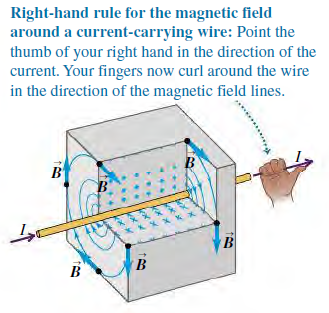
\includegraphics[width=\columnwidth]{Elektro/Figurer/right_hand_rule.PNG}
        \caption{Illustration af højrehåndsreglen for en lige leder. Kilde: figur 28.6 i \cite{youngSearsZemanskyUniversity2016}.}
        \label{fig:right_hand_rule_el}
    \end{subfigure}
    %
    \hfill
    %
    \begin{subfigure}[t]{.47\textwidth}
        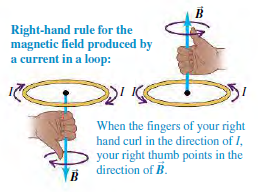
\includegraphics[width=\columnwidth]{Elektro/Figurer/right_hand_rule_loop.PNG}
        \caption{Illustration af højrehåndsreglen for en cirkulær leder. Kilde: figur 28.13 i \cite{youngSearsZemanskyUniversity2016}.}
        \label{fig:right_hand_rule_el_loop}
    \end{subfigure}
    \caption{Illustration af de to versioner af højrehåndsreglen til at finde retningen på et magnetfelt fra en leder.}
    \label{fig:right_hand_rule_both}
\end{figure}

\subsubsection{Højrehåndsreglen}
Det er vigtigt at bemærke at ligning \eqref{eq:b-felt_fra_punktladning} medfører at retningen er givet fra et krydsprodukt af ladningernes bevægelsesretning og en vektor fra ladningen. Højrehåndsreglen for krydsprodukter kan derfor bruges til at finde retninger på magnetfelter. Der er dog en anden højrehåndsregel, der giver samme resultater, som den fra afsnit \ref{fig:right_hand_rule_mat}, som er en fordel at bruge i dette tilfælde. Den fungerer ved at placere højre tommelfinger i strømmens retning eller ladningens bevægelses retning, hvorefter man krøller de andre fingre sammen. Magnetfeltet er så cirkulært om lederen i den retning fingrene peger, se figur \ref{fig:right_hand_rule_el}. Reglen kan også fungere den anden vej rundt, i tilfælde af cirkulær strøm, se figur \ref{fig:right_hand_rule_el_loop}.

\subsection{Amperes lov}
Begrænser man sig til jævne strømme,
%
\begin{align}
    \pdv{\va J}{t} = \pdv{\va I}{t} = 0,
\end{align}
%
viser det sig empirisk at Amperes lov gør sig gældende. Den siger at
%
\begin{align} \label{eq:ampere}
    \oint_P \va B \cdot \dd{\va{l}} = \mu_0 I_\mathrm{inde}.
\end{align}
%
Her angiver $\dd l$ at der er tale om det, der hedder et linjeintegral, hvilket betyder at man integrerer langs en fastlagt linje, og $I_\mathrm{inde}$ er den indesluttede strømstyrke. Den indesluttede strømstyrke er den strømstyrke, der løber igennem den løkke, som den linje man integrerer over. Bemærkelsesværdigt må man vælge en hvilken som helst linje at integrere over, så længe den er lukket, og derefter skal man bruge den tilsvarende strømstyrke. Den linje man integrere over kaldes en Ampereløkke. At Amperes lov er bevist empirisk betyder at de forudsigelser man kan lave med den stemmer overens med eksperimenter, og den kan derfor ikke som sådan udledes matematisk fra noget andet. Det er en abstrakt måde at skrive Amperes lov op, og det tjener det formål at den gælder i alle sammenhænge og i alle koordinatsystemer. For at få en forståelse af hvad det betyder, og hvordan man i praksis bruger ligning \eqref{eq:ampere}, så betragtes et eksempel.
%
\begin{figure}
    \begin{subfigure}{.47\columnwidth}
        \centering
        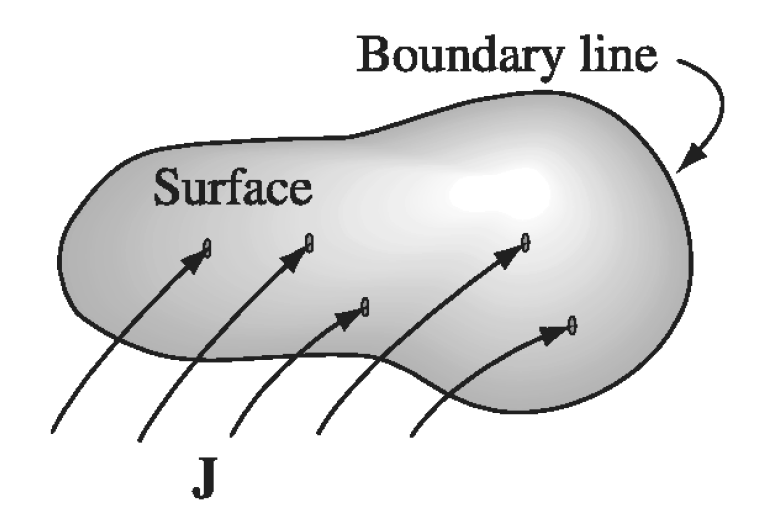
\includegraphics[width=\columnwidth]{Elektro/Figurer/ampere.PNG}
        \caption{Et arbitrært område, hvori der løber en strøm og dermed også en strømtæthed, som så er indrammet af en linje. Kilde: figur~5.31 i \cite{griffithsIntroductionElectrodynamics2017}.}
        \label{fig:ampere}
    \end{subfigure}
%
\hfill
%
    \begin{subfigure}{.47\columnwidth}
        \centering
        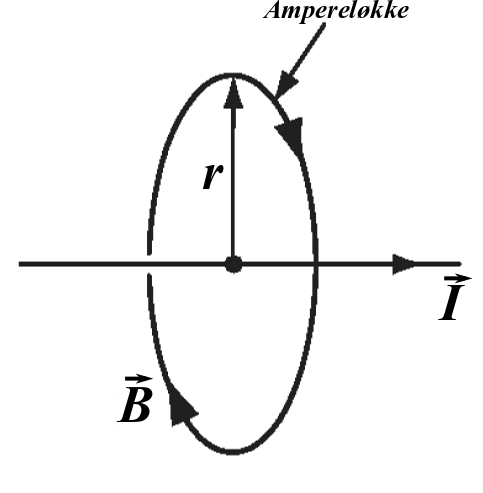
\includegraphics[width=.7\columnwidth]{Elektro/Figurer/lang_lige_leder.PNG}
        \caption{En strømstyrke $I$ løber igennem en uendelig lang lige leder og der placeres en ampereløkke. Kilde: figur~5.32 i \cite{griffithsIntroductionElectrodynamics2017}.}
        \label{fig:lang_lige_leder}
    \end{subfigure}
    \caption{ }
\end{figure}
%
\subsubsection{Den lange lige leder} \label{sec:lang_lige_leder}
Den lange lige leder er et klassisk eksempel på Amperes lov, hvor man bestemmer det magnetiske felt fra en uendelig lang og tynd lige leder overalt i rummet. I første omgang skal man vælge en ampereløkke, hvor der vigtige er at få den valgt så man gør integralet så let for sig selv som muligt. Af højrehåndsreglen fremgår det at magnetfeltet er cirkulært omkring ledningen, hvilket følger af antagelsen om at ledningen er uendelig lang. Hvis lederen ikke havde været uendelig lang ville feltet bøje af i nærheden af kanterne, man da noget uendeligt ikke har nogen kant, så kan feltet kun afhænge af afstanden til ledere - andet ville bryde cylindersymmetrien. Cirklen er smart som ampereløkke, da magnetfeltet så er parallelt med ampereløkken, hvorfor
%
\begin{align}
    \va B \cdot \dd{\va{l}} = B\dd{l},
\end{align}
%
altså blot en skalar og ikke en vektor. Af cylindersymmetrien er størrelsen af magnetfeltet uafhængigt af hvor på løkken man er, hvorfor $B$ er en konstant overfor integrationen:
%
\begin{align}
    \oint_P \va B \cdot \dd{\va{l}} = B \oint_P \dd{l}
\end{align}
%
Prikproduktet skal regnes inden feltet kan trækkes udenfor integralet, da integralet ellers ikke er veldefineret. Et lukket integral over en løkke er løkkens længde, hvilket i det her tilfælde er omkredsen af en cirkel. Yderligere er den indesluttede strøm $I_\mathrm{inde} = I$, hvorfor
%
\begin{align} \label{eq:lang_lige_leder}
    \mu_0I_\mathrm{inde} = B\oint_P \dd{l} = B \cdot 2\pi r  \Rightarrow  B = \frac{\mu_0I}{2\pi r}.
\end{align}
%
Det vigtige når man bruger Amperes lov er symmetri ligesom med Gauss' lov, \eqref{eq:GaussLawGeneral}, og det handler om fysisk at kunne argumentere for magnetfeltets retning overalt i rummet men også hvilke parametre styrken afhænger af og hvor denne er konstant.

\section{Induktion}
Magnetisk induktion er en proces, hvor en ændring i et magnetfelt skaber et elektrisk felt. Mere præcist skaber en ændring i et magnetfelt igennem en løkke et elektrisk felt i selve løkken, som får en strøm til at løbe. For at forstå det skal konceptet om magnetisk flux dog introduceres.

\subsection{Magnetisk flux}
I afsnit \ref{sec:elektrisk_flux} blev konceptet elektrisk flux introduceret som et overfladeintegral. Helt analog defineres den magnetiske flux som
%
\begin{align} \label{eq:magnetisk_flux}
    \Phi_B = \int_S \va B \cdot \dd \va a.
\end{align}
%
Det ses her at magnetisk flux minder meget om integralet i Amperes lov, \eqref{eq:ampere}, men med en meget vigtig forskel - fluxen er et overfalde integral, hvorfor det er et todimensionelt integral defineret ud fra overfladens normalvektor.

\subsection{Faradays lov}
Induktionen er matematisk beskrevet af Faradays lov, der siger at
%
\begin{align} \label{eq:faraday}
    \dv{\Phi_B}{t} = \dv{}{t} \int_S \va B \cdot \dd \va A = - \oint_P \va E\cdot \dd \va l = -\mathcal{E}.
\end{align}
%
$\mathcal{E}$ kaldes den \emph{elektromotoriske kraft} og er en spændingsforskel, som i kredsløbsanalyse ofte betegnes med $V$. %Igennem Ohms lov skaber spændingen en strømstyrke ud fra modstanden i kredsløbet $R$:
%
% \begin{align}
%     I = \frac{U}{R}.
% \end{align}
%
Når man regner induktion, er det også vigtigt, hvilken retning strømmen løber. Dette afgøres med endnu en højrehåndregel, hvor højre tommelfinger placeres i den retning magnetfeltets ændrer sig, hvorefter strømmen løber i den vej rundt i løkken resten af ens fingre peger. Denne højrehåndsregel kaldes Lenz' lov. Det er vigtigt at tommelfingeren placeres i den retning feltet ændrer sig, hvilket kan illustreres med et eksempel. Antag at magnetfeltet igennem en ring er vinkelret på ringens plan, hvilket kaldes $z$-retningen. Skrues der nu op for feltet, ændres det i positiv $z$-retning, hvorfor den inducerede strøm i ringen løber mod uret. I tilfældet hvor feltstyrken mindskes, skal ens tommenfinger pege i negativ $z$-retning, hvorfor den inducerede strøm løber med uret. Figur \ref{fig:right_hand_rule_both} kan derfor bruges, men med den krølle at man i begge figurer skal erstatte $B$ med $\dd{B}/\dd{t}$. \\
%
Det viser sig faktisk at ændringer i elektriske felter også inducerer magnetiske felter. Det hele kommer af at magnetiske felter er introduceret til at håndtere situationer med ladninger i bevægelse. Da felterne opfører sig ret forskelligt, troede man i lang tid også at elektricitet og magnetisme var to forskellige ting, men det viser sig at være to sider af samme sag. Speciel relativitetsteori, der introduceres i kapitel \ref{sec:rela}, beskæftiger sig med hvad der sker, når observatører bevæger sig i forhold til et eksperiment, og det viser sig at et magnetisk felt for en observatør i hvile, er det samme som et elektrisk felt for en observatør i bevægelse sammen med eksperimentet. Det er dog en historie for en anden gang.

\section{Lorentzkraften}
Når nu både elektrostatik (ladninger i hvile) og magnetostatik (ladninger i jævn bevægelse) er introduceret kan den elektriske og magnetiske kraft, ligningerne \eqref{eq:kraft_fra_e-felt} og \eqref{eq:magnetisk_kraft} samles til en elektromagnetisk kraft kaldet Lorenztkraften. Dette gøres med en sum ud fra superpositionsprincippet, der her siger at den totale kraft på et legeme er summen af hvert kraftbidrag. For en partikel med ladning $q$ og hastigheden $\va v$, der bevæger sig i et elektrisk felt $\va E$ og magnetisk felt $\va B$ er Lorentzkraften
%
\begin{align}
    F = q \Big(\va E + \va v \times \va B\Big).
\end{align}
%
Denne formel er relativt simpel og derfor handler store dele af elektromagnetisme om at beregne felterne - man har så at sige gemt det besværlige væk i nogle pæne symboler.
